\documentclass[a4paper,12pt,fleqn]{article}
\usepackage[utf8]{inputenc}
\usepackage[T1,T2A]{fontenc}
\usepackage[english,bulgarian]{babel}
\usepackage{amsfonts}
\usepackage{amssymb}
\usepackage{amsmath}
\usepackage{fullpage}
\usepackage{listings}
\usepackage{amsmath,amsfonts}
\usepackage{graphicx}
\usepackage{mathtools}
\DeclarePairedDelimiter\ceil{\lceil}{\rceil}
\DeclarePairedDelimiter\floor{\lfloor}{\rfloor}
\usepackage{tkz-graph} % from ctan or TL2011 one file tkz-graph.sty 

\lstset{language=C++,
	basicstyle=\ttfamily,
	keywordstyle=\color{blue}\ttfamily,
	stringstyle=\color{red}\ttfamily,
	commentstyle=\color{green}\ttfamily,
	morecomment=[l][\color{magenta}]{\#}
}


\title{Skip-List срещу AVL Tree}
\author{Стойчо Кьосев}
\date{June 2022}
\begin{document}
	\maketitle
	\textit{Въвеждаме структурите от данни Skip List и AVL дърво. Разглеждаме стандартните операции свързани с тях и техните сложности. Сравняваме ги и разглеждаме множество от тестове.}
	
	\section{AVL дърво}
	Двоично дърво наричаме всяко дърво с максимална разклоненост 2.
	За двоично наредено дърво ползваме следната рекурсивна дефиниция:
	\begin{enumerate}
		\item Празното дърво е двоично наредено дърво
		\item Стойностите в лявото поддърво са по - малки от стойностите в корена. Стойностите в дясното поддърво са по - големи от тези в корена. Лявото и дясното поддърво също са двоични наредени дървета.
	\end{enumerate}
	Височина на кореново дърво наричаме максималното разстояние между корена и което и да е листо.
	Двоично наредено дърво се наричаме балансирано ако височините в лявото и дясното поддърво се различават най - много с единица.\\
	За самобалансиращи дървета интуитивно можем да мислим като дървета, чиито операции запазват дървото балансирано.\\
	\\AVL дърветата са вид самобалансиращи се двоични дървета. Основните операции остават същите като в двоичните наредени дървета - търсене, добавяне на елемент и премахване на елемент. Разликата е, че при добавяне и премахване на елемент правим операции наречени дървесни ротации, които помагат да запазим дървото балансирано. 
	\\Нека с $n$ означаваме броя на елементите в дървото. Сложностите по време в най - лошия случай на стандартните операции, относно n, са следните:
	\begin{enumerate}
		\item Търсене: $O(\lg(n))$
		\item Добавяне на елемент: $O(\lg(n))$
		\item Премахване на елемент: $O(\lg(n))$
		\item Обхождане: $O(n)$
	\end{enumerate}
	Използват се четири вида ротации - лява, дясна, дясно-лява и ляво-дясна. При добавяне на елемент в AVL дърво можем да направим най - много 2 ротации. При изтриване на елемент обаче това не е така. Възможно е да направим до $\lg(n)$ ротации.\\
	Сложността по памет на AVL дървото е $O(n)$.
	\section{Skip-List}
	\textit{Skip lists are a data structure that can be used in place of balanced trees.
		Skip lists use probabilistic balancing rather than strictly enforced balancing
		and as a result the algorithms for insertion and deletion in skip lists are
		much simpler and significantly faster than equivalent algorithms for
		balanced trees.}\\
	\\Нека имаме стандартен свързан списък. За да намерим елемент е възможно да ни се наложи да претърсим целия лист. Ако имаме указатели към всеки втори елемент и листът е сортиран ще ни се наложи да претърсим $\frac{n}{2}$ елемента. Тук имаме горна граница от $\ceil*{\frac{n}{2}} + 1$ проверки, но все още това не подобрява търсенето асимптотично. Добре, нека имаме указатели към всеки четвърти елемент, запазвайки тези към всеки втори. Това влече горна граница от $\ceil*{\frac{n}{4}} + 2$. Това отново не подобрява сложността асимптотично, ни води до друга идея с която ще успеем! Нека неформално си представим някакви нива за търсене. Логично е, че първото ниво ще съдържа всеки елемент. Второто ще съдържа половината, третото една четвърт и така нататък. Това влече $\ceil*{\log_2{n}}$ горна граница за търсенето и вече имаме желаната асимптотика. Разбира се, в тези нива поддържаме елементите сортирани. Също така, сложността на добавянето и изтриването на елемент могат лесно да се имплементират с логаритмична сложност по броя на елементите в списъка.\\
	Структурата, реализирана грамотно, заема $O(n)$ памет ако приемем броя на нивата за константа предварително избрана от нас.\\
	В оригиналното представяне на структурата на всяко ниво авторът добавя още два елемента. Началния има ключ по - малък от всеки друг а крайния има ключ по - голям от всеки друг.\\
	Интуитивно представяне на Skip-List:
	% TIKZ-------------------------------------------------------------------------------------
	
	\begin{tikzpicture}
		\SetGraphUnit{1.5}
		\SetVertexNormal[Shape    = rectangle,MinSize=.8 cm]
		%%%%%%%%%%%%%%%%% vertices %%%%%%%%%%%%%%%%%%% 
		%  name of node x;y  x row y column
		
		\Vertex[L=$-\infty$] {0;0}
		
		\foreach \num [count=\n from 0] in  {1,2,3}
		{\NO[L=$-\infty$](0;\n){0;\num}}        
		% No = north (initial node) {new node}  L=label 
		\foreach \num/\label [count=\n from 0] in  
		{1/11,2/15,3/17,4/28,5/31,6/55,7/56,8/61,9/+\infty}
		{\EA[L=$\label$](\n;0){\num;0}} 
		\foreach \num [count=\n from 0] in  {1,2,3}{%
			\NO[L=$+\infty$](9;\n){9;\num}}  
		
		\foreach \num [count=\n from 0] in  {1,2,3} {%
			\NO[L=$31$](5;\n){5;\num}}   
		
		\foreach \no/\label  in  {1/11,2/15,6/55,7/56} {%
			\NO[L=$\label$](\no;0){\no;1} } 
		
		%%%%%%%%%%%%%%%%% edges %%%%%%%%%%%%%%%%%%%%%%%
		\foreach \num [count=\n from 1] in  {0,...,8}  {\Edge(\num;0)(\n;0)}
		
		\foreach \num [count=\n from 1] in  {0,...,2}  
		{\Edge(0;\num)(0;\n)  \Edge(5;\num)(5;\n)  \Edge(9;\num)(9;\n)}
		
		\foreach \num  in  {1,2,6,7} {\Edge(\num;0)(\num;1)}   
		
		\foreach \num [remember=\num as \lastnum (initially 0)] in  {5,9}  
		{\Edge(\lastnum;3)(\num;3) }  
		
		\foreach \num [remember=\num as \lastnum (initially 0)] in  {5,9}  
		{\Edge(\lastnum;2)(\num;2)} 
		
		\foreach \num [remember=\num as \lastnum (initially 0)] in  {1,2,5,6,7,9}  
		{\Edge(\lastnum;1)(\num;1)}     
	\end{tikzpicture}   
	% !TIKZ-----------------------------------------------------------------------------------
	\\Въпреки, че не навлизаме в детайлни обяснения за това как са реализирани алгоритмите а само разглеждаме техните сложности си струва да споменем, че Skip-List-ът е вероятнсотна структура от данни. При добавяне на нов елемент всеки път избираме на случаен принцип на кое ниво да го раплоложим. Разбира се, шансът да го разположим на първото е 100\%. За второто този шанс е 50\% и т.н. Това реално ни изправя пред шанс да имаме елементи само в първото ниво. В следващата част ще проверим практически дали нашата идея работи и ако да колко точно ефикасна е тя.
	
	\section{Тестове}
	Тестове в подсекции 3.1, 3.2 и 3.3 се изпълняват в release mode и са компилирани под MSVC на windows 11. Използваме процесор Intel Core i5 10th gen и разполагаме с 8GB рам.\\
	Реализациите на двете структури можете да намерите на следния адрес:\\
	\textit{https://github.com/stoychoX/AVL-vs-SkipList}
	\\Тестовете в които говорим за "това се изпълни за толкова време" са направени чрез класът Timer намиращ се в папката Benchmark.\\
	\\В папката за AVL дървото се съдържат тестове за коректност, които се стремят да провeрят дали стандартните операции запазват всички AVL инварианти. 
	Това обаче са тестове касаещи коректността на структурата и нямат място тук. Следващата подсекция представя множество от тестове, който също до някаква степен касаят коректността на Skip-List-a. Тя намира място тук понеже смятам, че е интересна.
	\subsection{Бърка ли наистина Skip-List-a}
	Разглеждаме следния код:
	\begin{lstlisting}
	SkipList<int> sl;
	for (size_t i = 0; i < 10000; i++)
		sl.insert(i);
	sl.print();
	\end{lstlisting}
	Метода print() ни извежда на конзолата колко елемента имаме във всяко ниво, като започваме от най - горното. По конвенция нашия списък има 6 нива. Това може да се промени, но нека за тестът го оставим така. Изходът от този фрагмент е:
	(335, 637, 1232, 2528, 5052, 10000)
	\\Виждаме, че да, разпределението не е максимално точно, но е повече от достатъчно добро!\\
	След 100 теста нещата се запазват:
	
	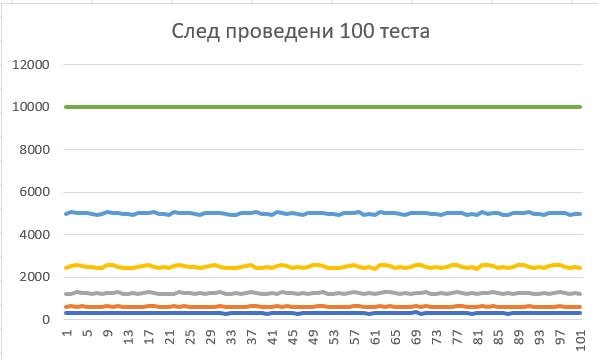
\includegraphics[scale=0.45]{insert-tests.jpg}\\
	Въпреки теоретичната вероятност да имаме "лошо" разпределение на елементите, това не се случва.
	\subsection{Зареждане и търсене}
	Нека проверим колко добре се справят двете структури при зареждане и търсене на информация. За теста ще заредим речникът на оксфорд - дума по дума. Разбира се, ще изключим повтарящите се думи. В Skip-List класът позволяваме да има повтарящи се елементи. Това не е случая с AVL дървото обаче. Та тестовете ще се извършват върху колекции с различни елементи. Файлът върху който работив е с размер 1064KB.\\
	Какво показват резултатите:\\
	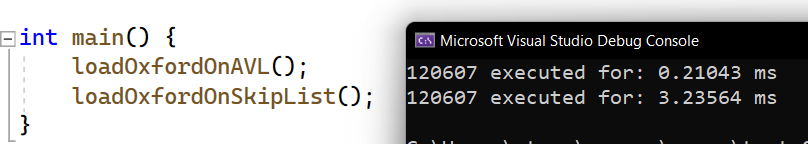
\includegraphics[scale=0.4]{oxford-load.png}\\
	От ляво виждаме, че и в двете структури има еднакъв брой елементи. AVL дървото побеждава Skip-List-a. Дали обаче това няма нещо общо с нивата? Работим с шест нива по подразбиране. Нека опитаме какво ще стане ако имаме 12.\\
	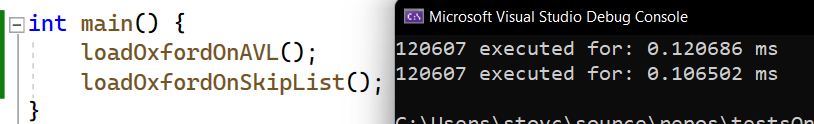
\includegraphics[scale=0.4]{oxford-load-2.png}\\
	С 12 нива вече победихме, въпреки че с много малко. Естественото нещо което можем да направим е да добавим още нива. Дали ако работим с 24 нива няма да "смажем" дървото?\\
	Пускаме тестът, но този път имаме 24 нива. Резултатът е до някъде очакван. Не го смазахме:\\
	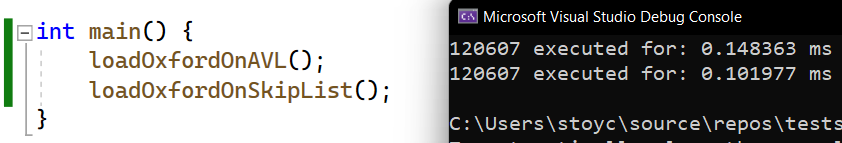
\includegraphics[scale=0.4]{oxford-load-3.png}\\
	Тоест да - има нещо като оптимален брой нива, но безразборното уваличаване на нива не ни влече безкрайно бърза структура. Перфектния брой на нивата е приблизително $\log(n)$.\\
	Какво става с паметта? Тук AVL дървото побеждава. При зареждане на данните на дървото му отнема около 9 MB докато листът заема около 13.\\
	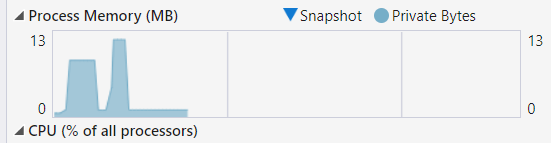
\includegraphics[scale=0.4]{mem-consume.png}\\
	Все пак до момента имаме следните резултати - ако нивата на SkipList-а са оптимални имаме горе-долу еднакво време за построяване. Дали си струва обаче допълнителната памет?\\
	Нека проверим какво се случва при търсенето. Нека търсим случайни стрингове. За всяка от двете структури ще направим $1*10^6$ заявки за търсене на случаен стринг.\\
	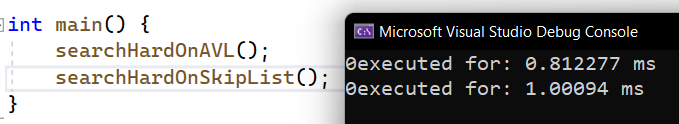
\includegraphics[scale=0.4]{search.png}\\
	Тук дървото побеждава. Но колко често ни се налага да търсим неща, които не съществуват? Теста е интересен но безполезен ако не видим какво ще стане ако търсим елементи, които са част от нашата колекция.\\
	Нека в обикновен вектор заредим напълно легално притежаваната от нас книга на J. K. Rowling Harry Potter, отново в .txt формат дума по дума. За всеки елемент на вектора ще търсим дали тази дума е в нашата колекция. Файлът е с размер 496KB.\\
	Ще изпълним следния код:\\
	\begin{lstlisting}
		for(int i = 0; i < 100; i++)
			searchHarryOnAVL();
		std::cout << std::endl;
		for(int i = 0; i < 100; i++)
			searchHarryOnSkipList();
	\end{lstlisting}
	Ще вземем резултатите от 100-те търсения и ще ги анализираме.\\
	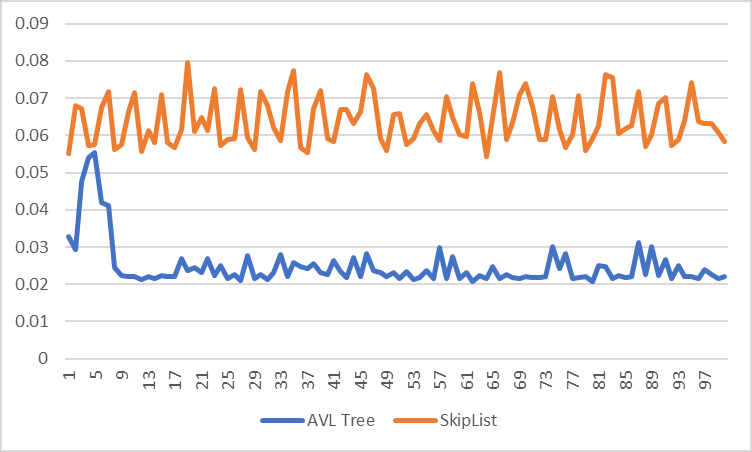
\includegraphics[scale=0.5]{searches.png}\\
	На око можем да кажем, че дървото приключва приблизително за 0,025 секунди а листът за приблизително 0,065. Нека погледнем как точно изглежда алгоритъмът за търсене в листа:\\
	\begin{lstlisting}[
		basicstyle=\tiny
		]
		template<class T, unsigned maxLevel>
		bool SkipList<T, maxLevel>::containsElement(const T& elem) const {
			NodeBase* it = header;
			
			for (int i = maxLevel - 1; i >= 0; --i) {
				while (it->forward[i] && it->forward[i]->value < elem) {
					it = it->forward[i];
				}
			}
			it = it->forward[0];
			return (it && static_cast<Node*>(it)->value == elem);
		}
	\end{lstlisting}
Самият каст от NodeBase* към Node* добавя допълнително натоварване при нашето търсене. Та можем да кажем, че двете структури се справят сравнително еднакво с поставената задача игнорирайки спецификите на реализацията.

\subsection{Конкурентност}
Представянето на двете структури до момента е сравнително еднакво. Дървото изразходва по - малко памет, но разликата не е твърде драстична. Голямото предимство на дърветата е тяхната моделираща мощ. Дървовидната структура е някак по - интуитивна, по - позната и познавайки тази структура можем лесно и бързо да решаваме голям клас задачи.\\
Защо бихме избрали Skip-List пред познатото ни дърво обаче? В многонишковото програмиране този тип свързани списъци се оказват предпочитани пред дърветата.
Оказва се, че можем да направим такъв тип свързан списък, който има по - висока производителност в многонишкова среда от двоично дърво за търсене. Конкурентните двоични дървета за търсене не са нещо често срещано. Интересен факт е, че червено черното дърво е измислено през далечната 1972 година. Конкурентно червено черно дърво обаче се появява чак през 2011 година.\\
Ref: http://www.cs.umanitoba.ca/~hacamero/Research/RBTreesKim.pdf\\

\subsection{Benchmark}
Добра идея би било да пуснем benchmark върху тестовете които направихме досега. Така ще разберем колко добре сме се справили с тях и също можем да надникнем в малко по - интересни детайли.\\
Използваме google benchmark. В тази секция тестовете са правени на виртуална машина VirtualBox работеща с Ubuntu. Машината разполага с 3 ядра, 4GB рам и 10GB физическа памет.\\
Отново пускаме подобни тестове, които се стремят да разгледат инициализиране и търсене. Ето Тестовете не са същите а са доста по - леки, понеже разполагаме с ограничено количество памет на виртуалната машина. Както видяхме в по -  горните секции само инициализацията ни задели около 13GB памет, с които тук просто не разполагаме. Също така кодът на тестовете е качен като оригиналните тестове са доста подобни.\\
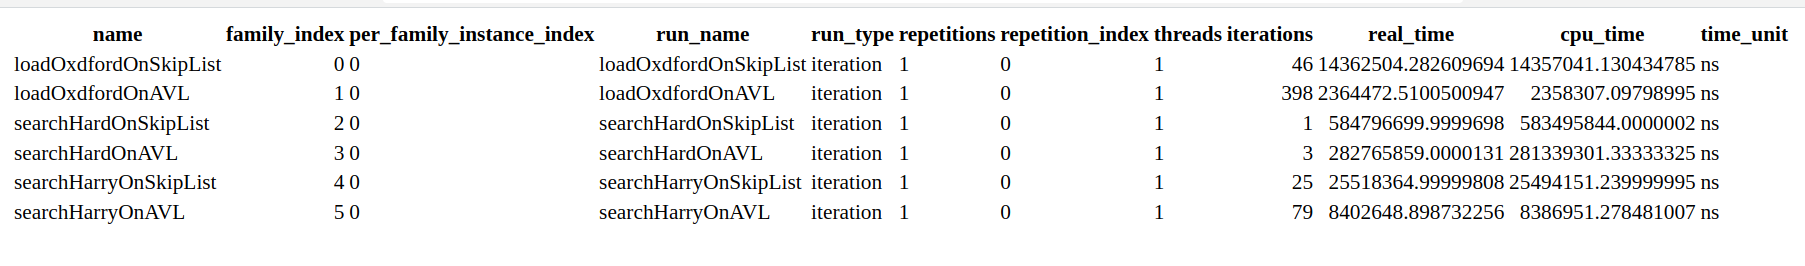
\includegraphics[scale=0.25]{html-final.png}\\
HTML документа представящ тази таблица е в папката Comparison.

\begin{thebibliography}{9}
\bibitem{texbook} Skip Lists: A Probabilistic Alternative to Balanced Trees by W. Pugh

\bibitem{lamport94} A Skip List CookBook

\bibitem{lamport94} Диаграма на Skip-List: https://tex.stackexchange.com/questions/22083/how-do-i-draw-extendible-hashing-skip-list-diagrams-using-tikz-library
\end{thebibliography}

\end{document}
